% Chapter Template

\chapter{Resultados} % Main chapter title

En este cap\'itulo  describiremos los datos utilizados en 	nuestros experimentos, las m\'etricas de calidad utilizadas para evaluar los resultados, la manera en la que se  utilizaron los datos y los resultados obtenidos.\\

En la secci\'on  4.1 se describen los materiales utilizados para la realizaci\'on de este trabajo final. Los tipos de dataset utilizados con las caracter\'isticas correspondientes a cada tipo de im\'agenes, dispositivos de captura, resoluci\'on de las im\'agenes, entre otras.\\

En la secci\'on 4.2  se estudian las m\'etricas de calidad utilizadas..\\

En la secci\'on 4.3 se exponen los resultados obtenidos durante el dise\'no del algoritmo..\\

En la secci\'on 4.3.1 se exponen y analizan los resultados obtenidos durante la etapa de preprocesamiento. \\

En la secci\'on 4.3.2 ..\\

En la secci\'on 4.3.3 ..\\

En la secci\'on 4.4 ..\\

En la secci\'on 4.5 ..\\



\label{Chapter4} % Change X to a consecutive number; for referencing this chapter elsewhere, use \ref{ChapterX}

%----------------------------------------------------------------------------------------
%	SECTION 1
%----------------------------------------------------------------------------------------

\section{Materiales}

Para la realizaci\'on de este trabajo final se utilizaron 3 bases de datos con im\'agenes de fondo de ojo, DRIVE, HRF, ARIA.\\

DRIVE es una base de datos a disposici\'on del p\'ublico, que consta de un total de 40 im\'agenes a color con diferentes lesiones. Las fotograf\'ias se obtuvieron a partir de un programa de cribado de la retinopat\'ia diab\'etica en los Pa\'ises Bajos. La poblaci\'on de selecci\'on consisti\'o en 453 sujetos de entre 31 y 86 a\~nos de edad. Cada imagen se ha comprimido JPEG, lo cual es una pr\'actica com\'un en los programas de cribado. De las 40 im\'agenes en la base de datos, 7 contienen la patolog\'ia, es decir, los exudados, hemorragias y cambios del epitelio pigmentario. Ver (\ref{fig:Drive_images_retinal}) para un ejemplo de una imagen patológica y una normal. Las im\'agenes fueron adquiridas mediante una c\'amara no midriática de 3 CCD Canon CR5 con un campo de $45^{\circ}$ de visi\'on (FOV). Cada i\'agen es capturada utilizando 8 bits por plano de color a 768 {x} 584 p\'ixeles. El FOV de cada imagen es circular con un di\'ametro de aproximadamente 540 p\'ixeles. El conjunto de 40 im\'agenes se dividi\'o en un conjunto de prueba y entrenamiento, ambos contienen 20 im\'agenes. Tres observadores, el primer y segundo autor y un estudiante de inform\\'atica segmentaron manualmente un n\'umero de im\'agenes. Todos los observadores fueron entrenados por un oftalm\'ologo con experiencia. El primer observador segment\'o 14 im\'agenes del conjunto de entrenamiento, mientras que el segundo observador segment\'o las otros 6 im\'agenes. El equipo de prueba fue segmentado en dos ocasiones resultando en un conjunto X e Y. El conjunto X fue segmentado tant por el primer y segundo observador (13 y 7 im\'agenes, respectivamente), mientras el conjunto Y se segmentó por completo por el tercer observador. El rendimiento de los algoritmos de segmentaci\'o de los vasos se midi\'o en la prueba. En el conjunto X los observadores marcaron 577,649 p\'ixeles como vasos y 3.960.494 como fondo (recipiente de 12,7\%). En el conjunto Y 556,532 p\'ixeles se marcaron como vasos y 3.981.611 como fondo (recipiente de 12,3\%).\\


\begin{figure}[H]
	{
	\centering
	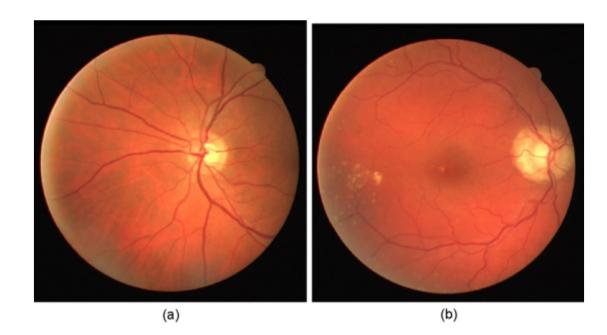
\includegraphics[width=1\textwidth]{Figures/Drive_images_retinal}
	\caption[Drive]{Im\'agen de la retina - DRIVE: (a) Retina saludable, (b) Retina con muestras patol\'ogicas.}
	\label{fig:Drive_images_retinal}
	}
\end{figure}	


HRF es una base de datos que ha sido establecida por un grupo de investigaci\'on sobre el reconocimiento de patrones, en un proyecto llevado a cabo por el laboratorio de la Universidad de Erlangen-Nuremberg Alemania  en cooperación con  la Clínica de Oftalmología Tomas de Kubena, Zlin, República Checa, para apoyar los estudios comparativos sobre los algoritmos de segmentaci\'on autom\'atica de im\'agenes en la retina del fondo del ojo. Es una base de datos a disposici\'on del p\'ublico, que contiene en este momento 15 im\'agenes de pacientes sanos, 15 im\'agenes de pacientes con retinopat\'ia diab\'etica y 15 im\'agenes de pacientes con glaucoma. Las im\'agenes segmentadas de los vasos est\'an disponibles para cada imagen. Tambi\'en se proporcionan las m\'ascaras, se determina el campo de visi\'on (FOV) para los conjuntos de datos particulares. Los datos est\'adar de oro son generados por un grupo de expertos que trabajan en el campo de an\'alisis de im\'agenes de la retina y los m\'edicos de las cl\'inicas oftalmol\'ogicas. Las im\'agenes se capturaron usando una c\'amara  Canon EOS-20D con un campo de visi\'on de $60^{\circ}$ FOV. 
El tama\~no de las im\'agenes es de 3504 {x} 2336 p\'ixeles. Todas las im\'agenes son de 24 bits por p\'ixel y son almacenada en formato JPEG.Se proporciona tambien para cada imagen, una máscara binaria para determinar el campo de visi\'on. \cite{budai2011public} \\

\begin{figure}[H]
\centering
\graphicspath {Figures} 
	  \label{fig:color}}
		\subfloat{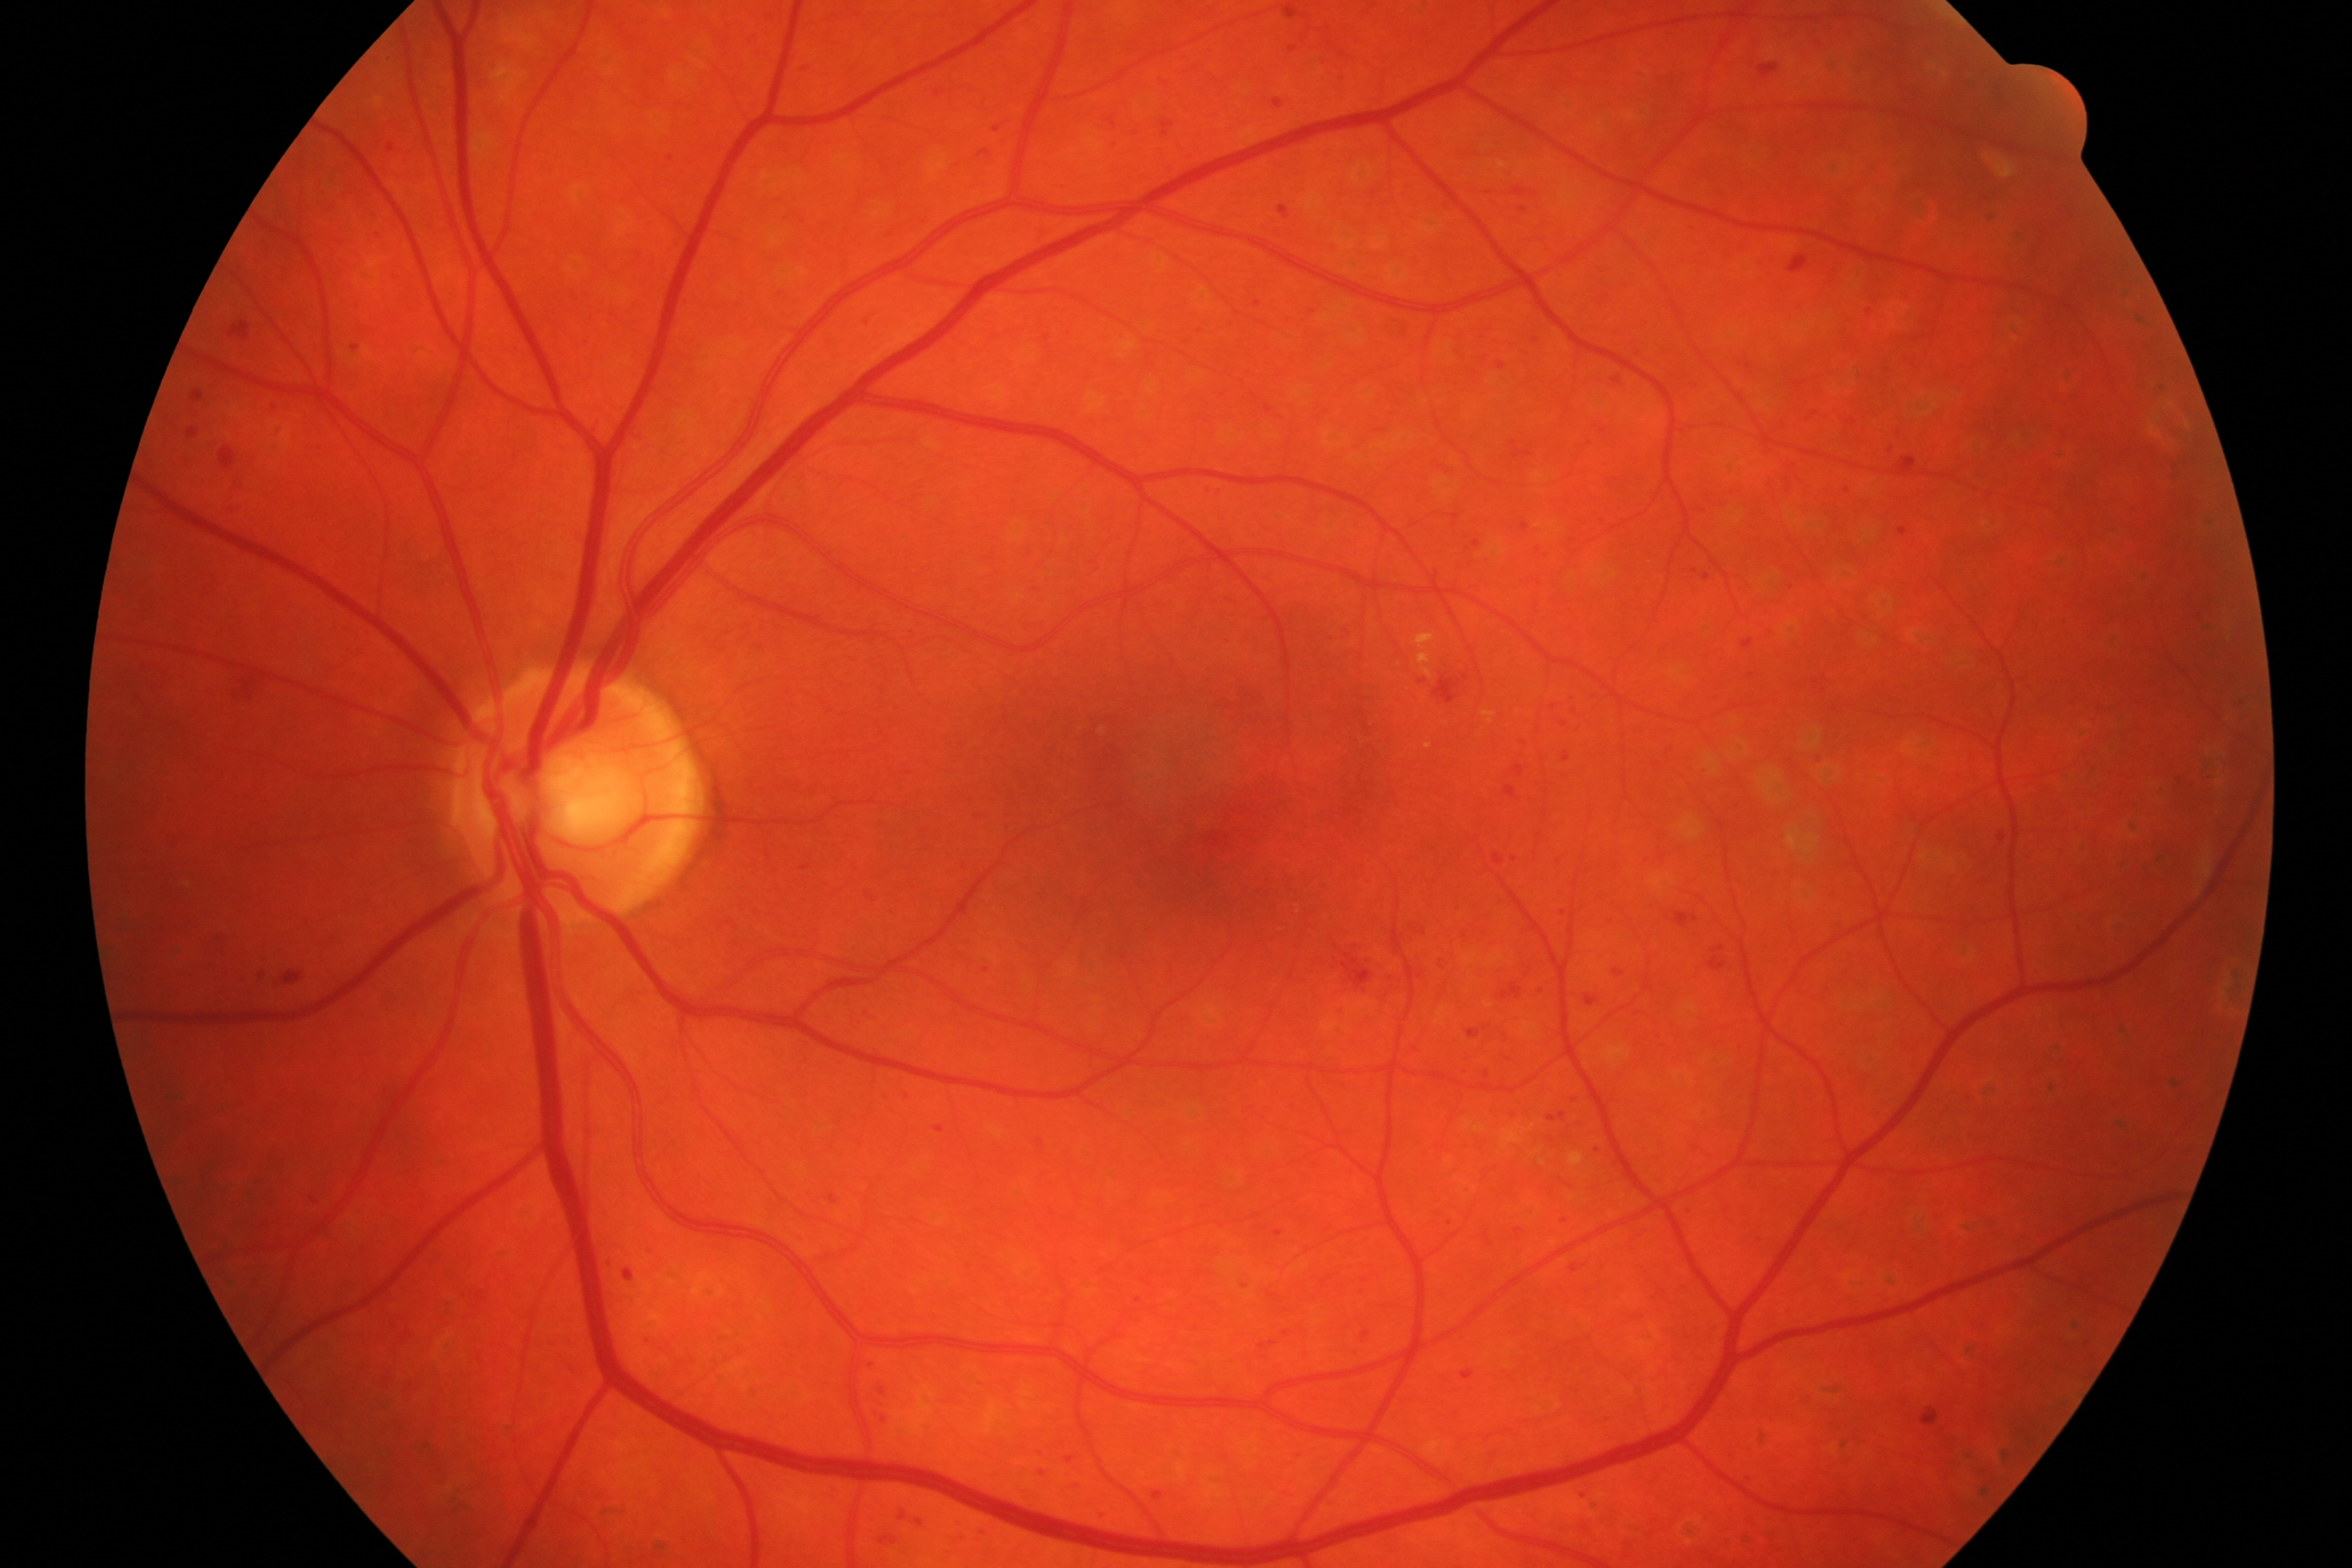
\includegraphics[width=0.3\textwidth]{01_dr.jpg} \label{fig:retinopatia}}
		\subfloat{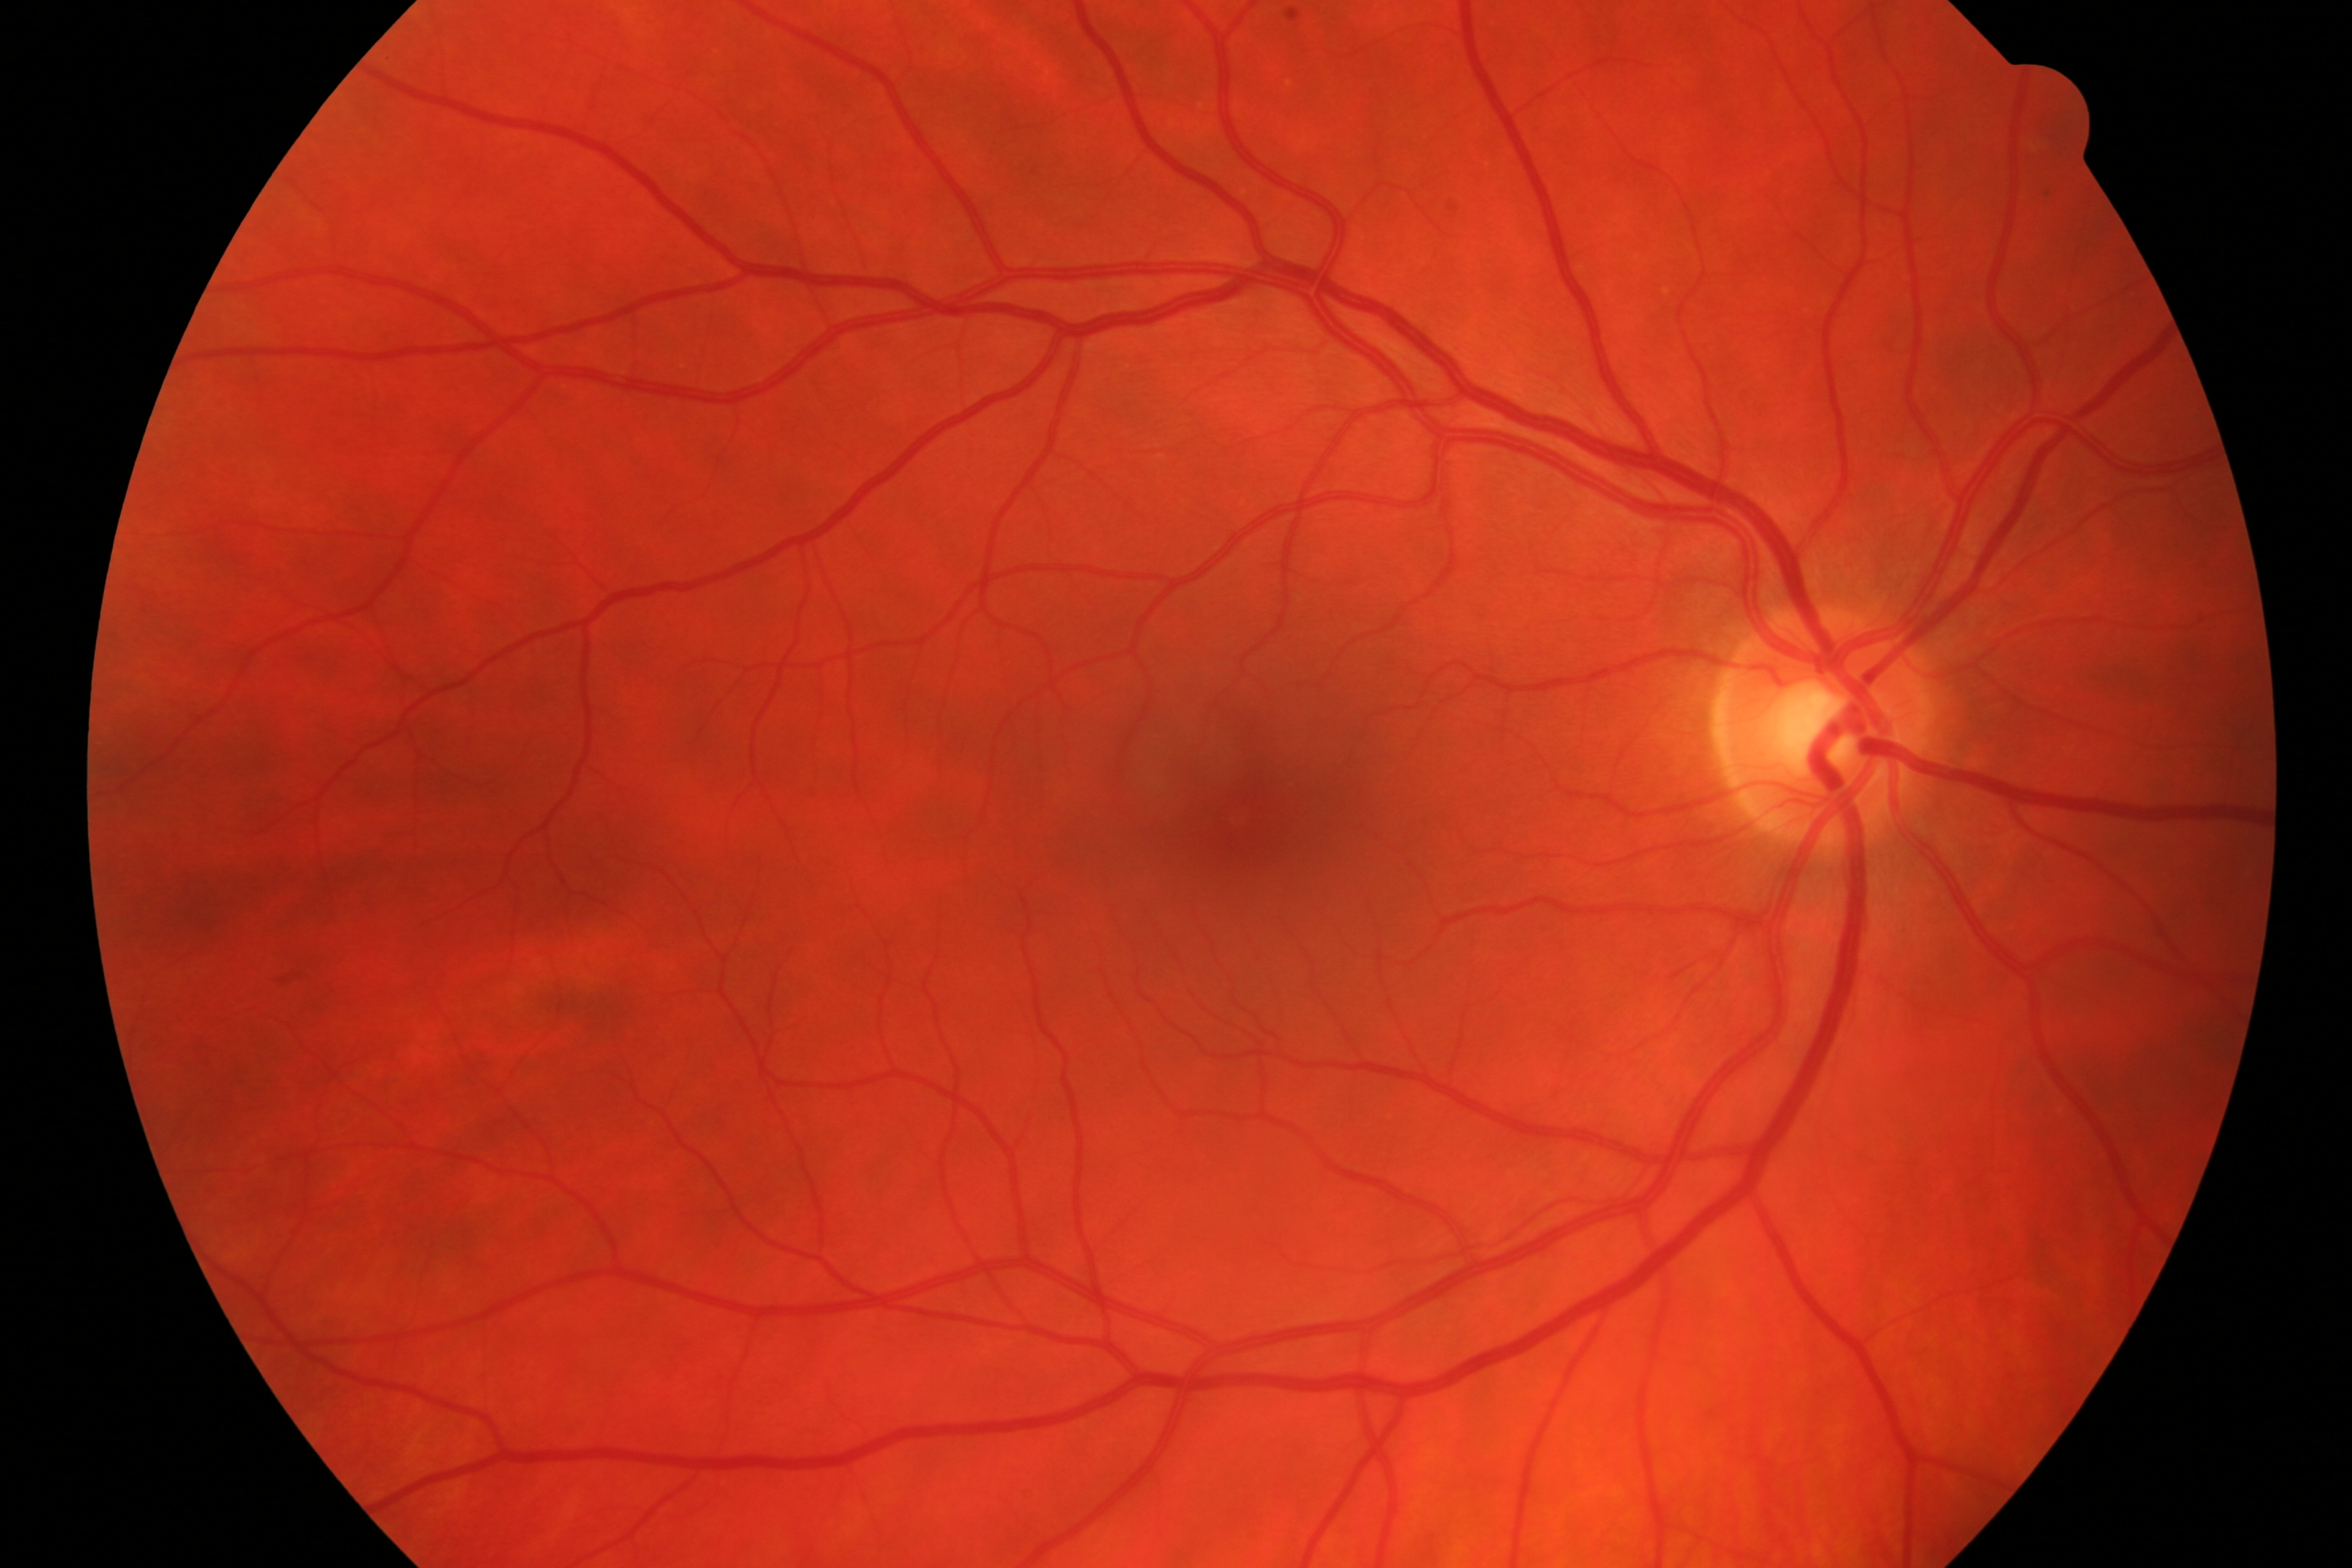
\includegraphics[width=0.3\textwidth]{01_g.jpg} \label{fig:glaucoma}}
		\subfloat{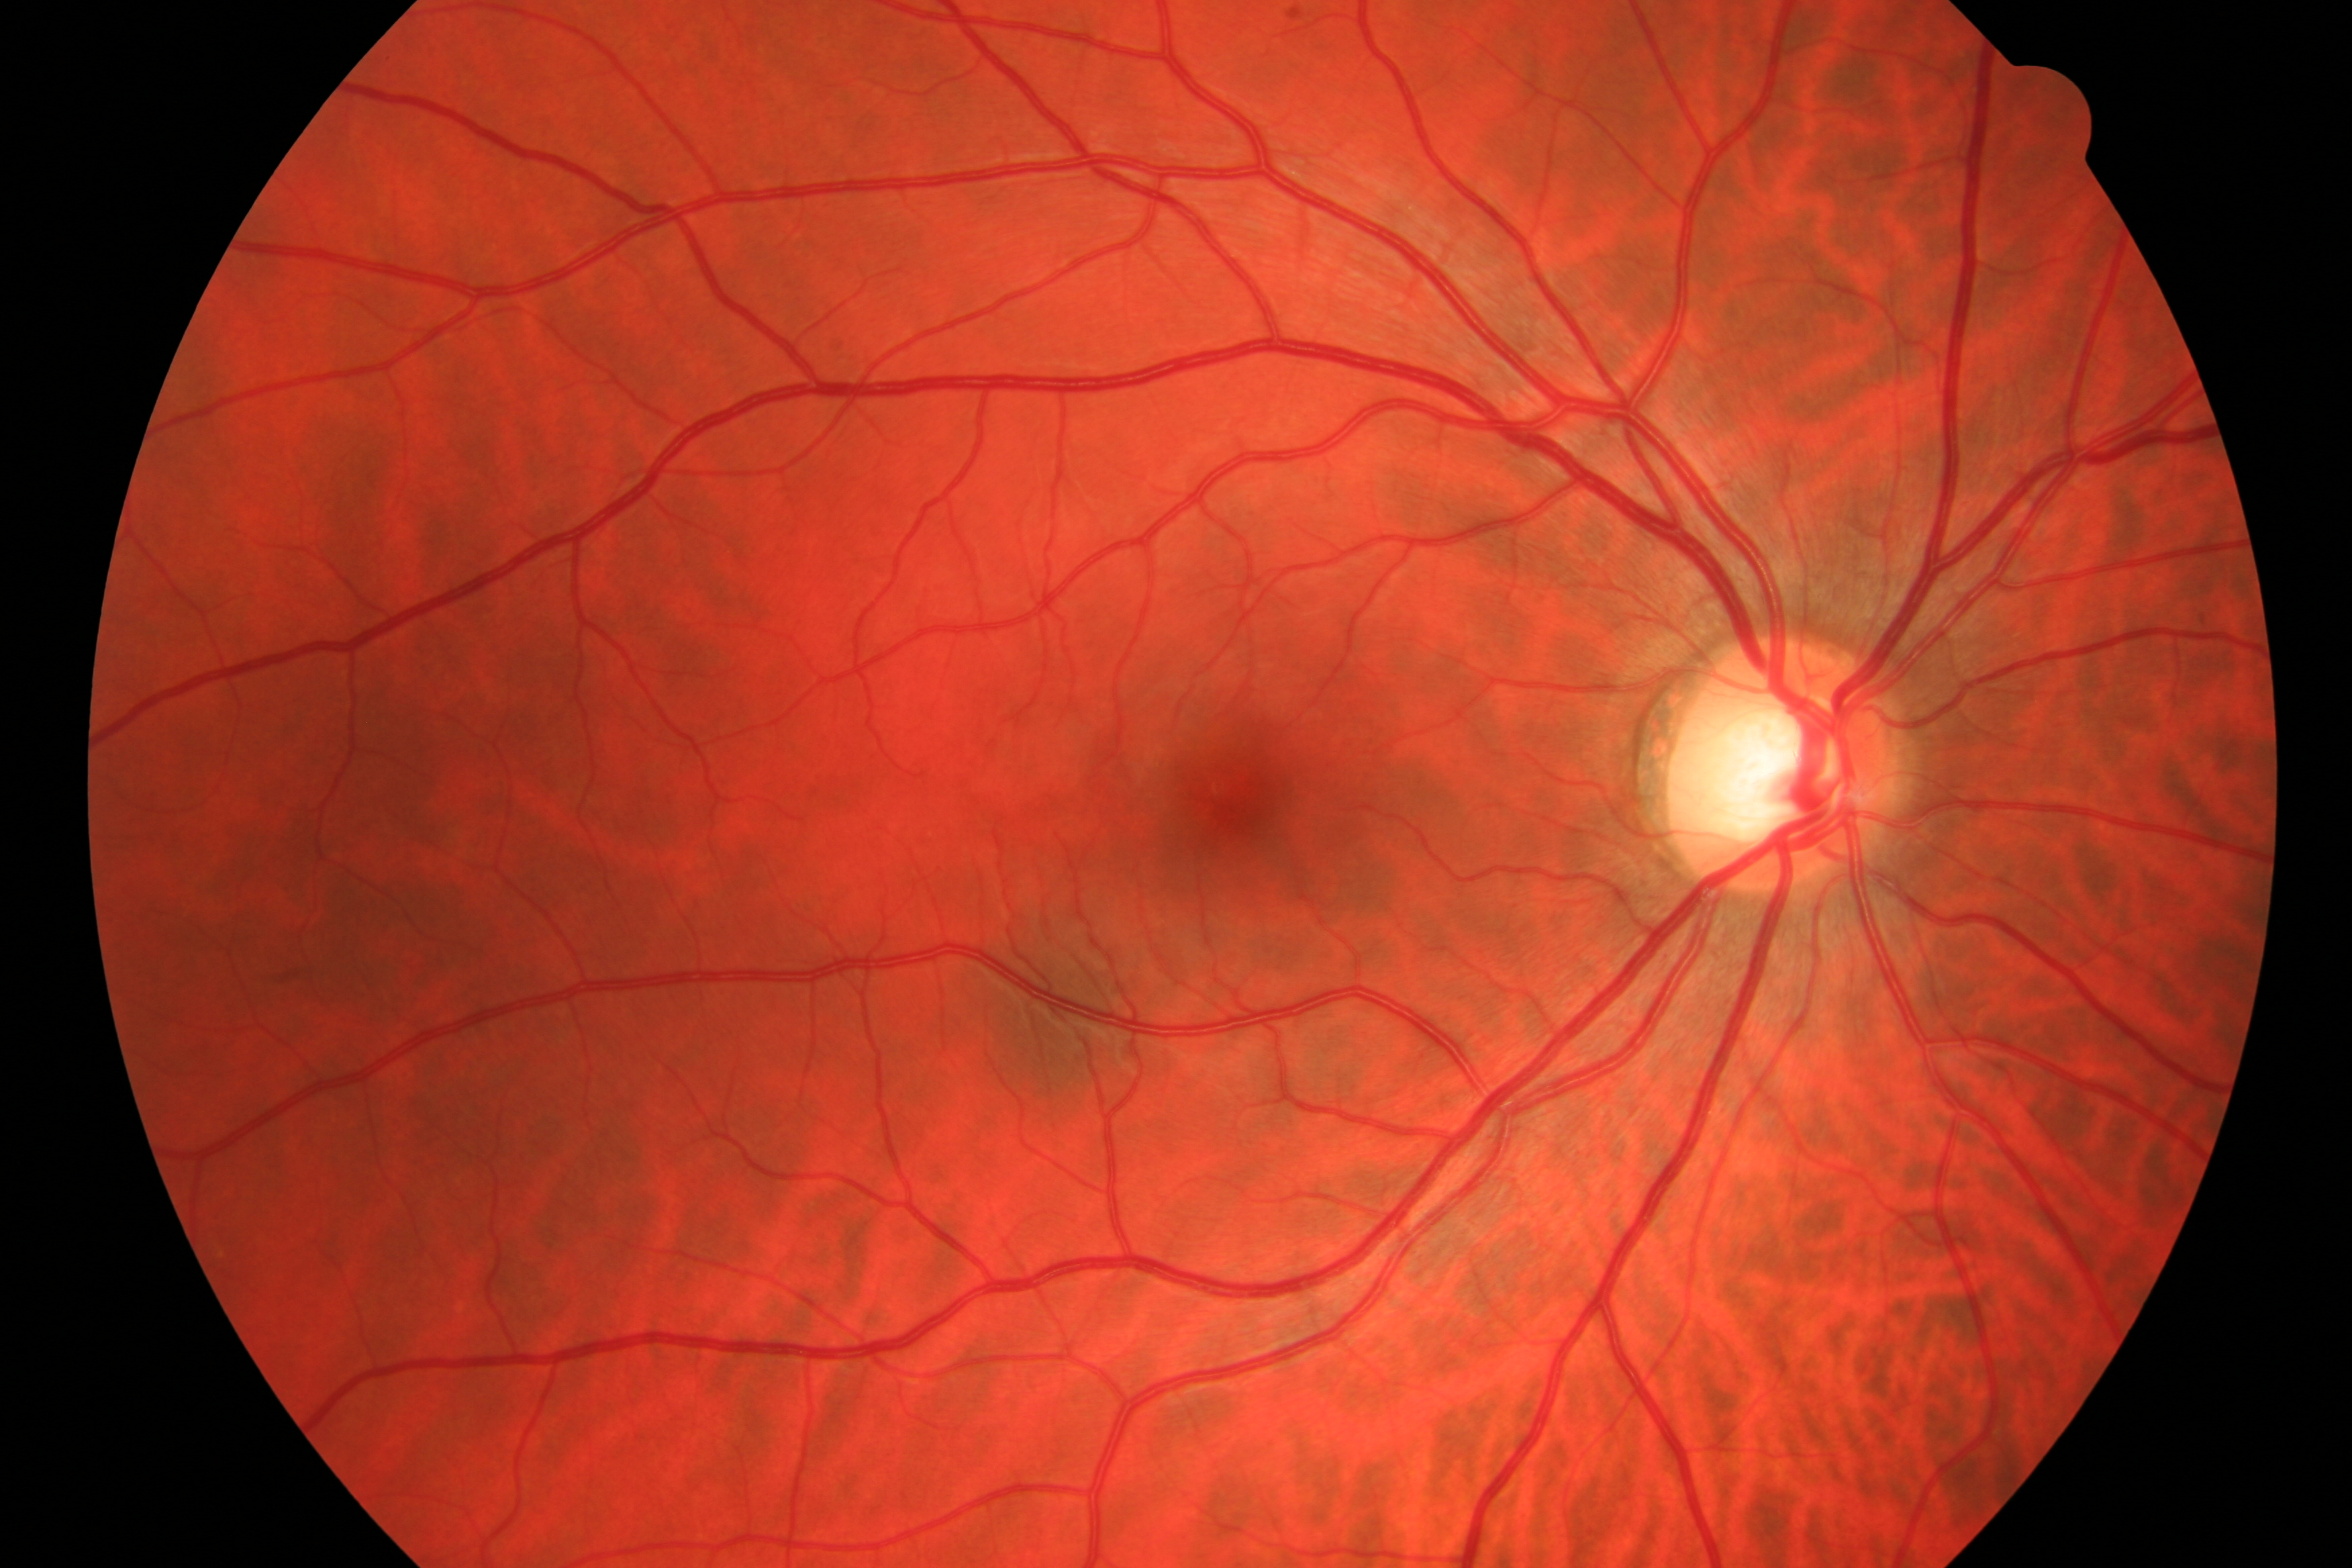
\includegraphics[width=0.3\textwidth]{01_h.jpg} \label{fig:sana}}
    \caption{Im\'agenes del dataset HRF. De izquierda a derecha: Retinopat\'ia  diabetica; Glaucoma; Imagen Sana}
		\label{fig:transferOverfeat}
\end{figure}

ARIA es una base de datos creada en 2006, en una colaboración de investigación entre  St. Paul's Eye Unit, Royal Liverpool University Hospital Trust, Liverpool, Reino Unido y el Departamento de Oftalmología, Ciencias Clínicas, Universidad de Liverpool, Liverpool, Reino Unido \cite{}. La base de datos consta de tres grupos; uno tiene 92 im\'agenes con degeneraci\'on macular relacionada con la edad, el segundo grupo tiene 59 im\'agenes con diabetes y un grupo de control se compone de 61 im\'agenes. El rastro de los vasos sangu\'ineos, la ubicaci\'on del disco \'optico y la f\'ovea est\'a marcada por dos expertos en an\'alisis de imagen como patr\'on de referencia. Las im\'agenes se capturan a una resoluci\'on de 768 {x} 576 p\'ixeles de colores RGB con 8 bits por plano de color con una c\'amara de fondo Zeiss FF450 con un campo de visi\'on de $50^{\circ}$ y se almacenan como archivos TIFF sin comprimir.\\

\begin{figure}[H]
\centering
\graphicspath {Figures} 
	  \label{fig:color}}
		\subfloat{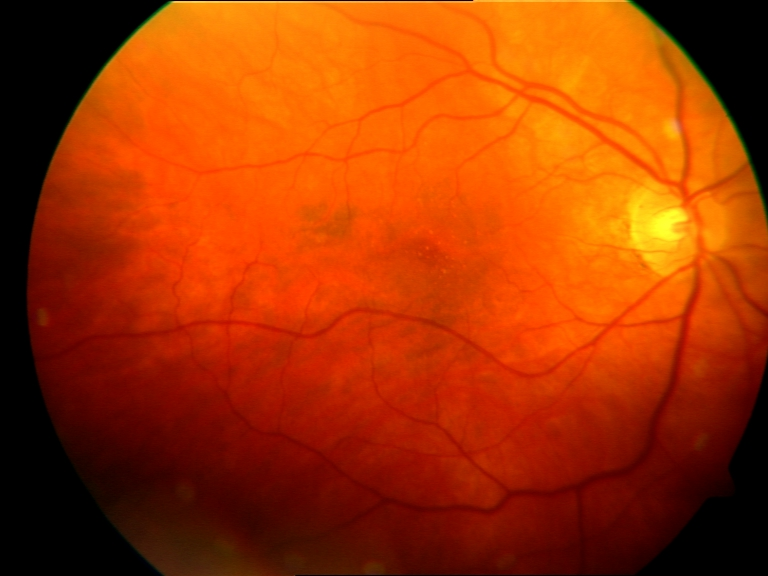
\includegraphics[width=0.3\textwidth]{a_01.png} \label{fig:a_}}
		\subfloat{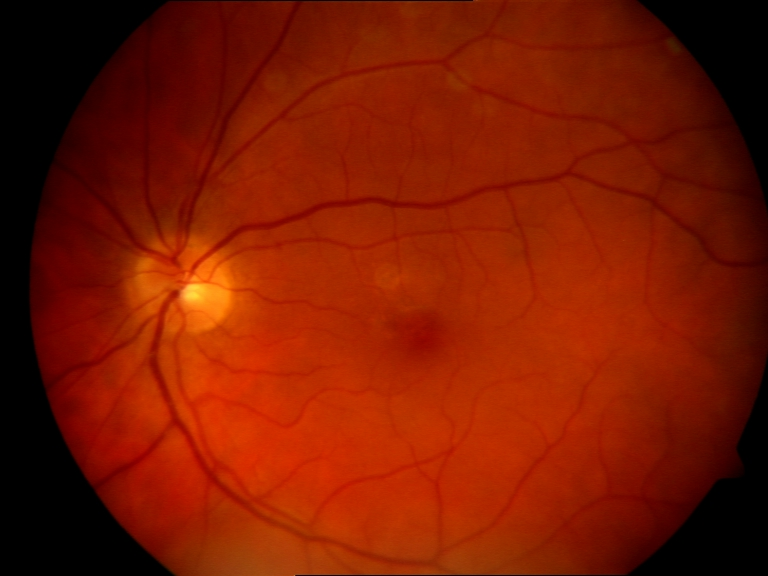
\includegraphics[width=0.3\textwidth]{c_1_7.png} \label{fig:c_}}
		\subfloat{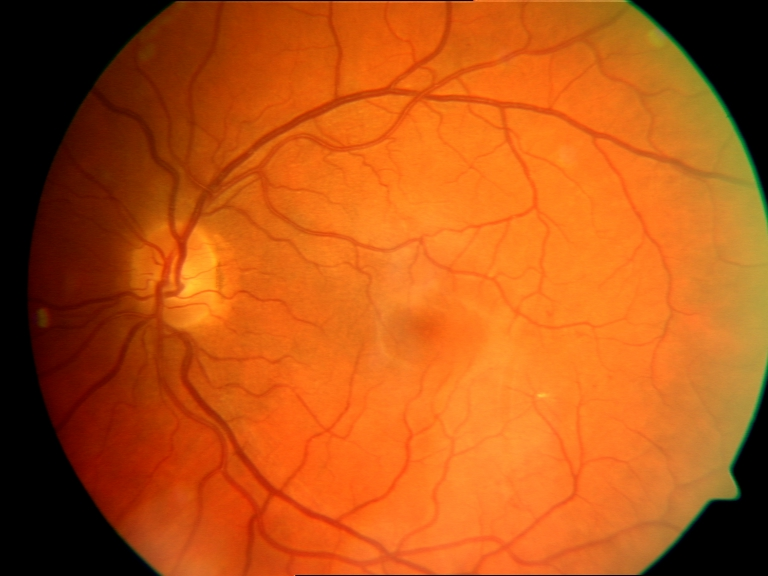
\includegraphics[width=0.3\textwidth]{d_1_19.png} \label{fig:d_}}
    \caption{Im\'agenes del dataset ARIA. De izquierda a derecha: a; c; d}
		\label{fig:transferOverfeat}
\end{figure}

%-----------------------------------
%	SECTION 2
%-----------------------------------
\section{M\'etricas de calidad utilizadas}


%-----------------------------------
%	SECTION 3
%-----------------------------------

\section{Resultados obtenidos durante el dise\'no del algoritmo}

%----------------------------------------------------------------------------------------
%	SECTION 4
%----------------------------------------------------------------------------------------

\subsection{Preprocesamiento}
\begin{itemize}
\item Extracci\'on de fondo: El objetivo de esta etapa consiste en suavizar la im\'agen, para esto calculamos el fondo de la misma, luego  restamos a la im\'agen original este fondo y de esta manera podemos remover el efecto de bias causado por la modalidad de captura de la im\'agen. Finalmente se convierte la im\'agen a double para tener mayor precisi\'on en las pr\'oximas etapas.
	\begin{itemize}
		\item Filtro de Mediana: para el calculo del filtro de mediana, se busc\'o cual era la mejor ventana a utilizar para cada uno de los dataset nombrados anteriormente, basandonos en el valor obtenido por la funci\'on vlroc de Matlab que determina el \'area bajo la curva promedio para cada set de im\'agenes. Los resultados arrojaron diferentes valores para cada conjunto de im\'agenes, por un lado se obtuvo un valor de ventana igual a 113 para el dataset HRF, lo cual es razonable para el tama\'no de dichas im\'agenes. Con este valor de ventana se obtuvo un \'area promedio de 0.xxxx.... Por otro lado, con el conjunto de DRIVE se determin\'o que el mejor valor de ventana es 29, dando un valor de \'area bajo la curva de 0.xxxx..,  lo cual tambi\'en es razonable ya que este tipo de im\'agenes son de menor tama\~no que las anteriores. Finalmente las im\'agenes ARIA resultaron un valor de ventana igual a 41 con un valor de \'area bajo la curva de 0.xxxx. IMAGENES DE LA CURVA DE ROC.
		\item Filtro Gaussiano: para el calculo de \'area bajo la curva de este filtro, se utilizaron los par\'ametros por defecto del filtro, observ\'andose que los valores obtenidos fueron muy por debajo de los obtenidos en los otros filtros. Por tal raz\'on se determin\'o que no es un filtro aplicable a este tipo de im\'agenes ya que no genera resultados buenos. IMAGENES DE LA CURVA DE ROC
		\item Filtro Promedio: para el calculo del filtro promedio, se busc\'o cual era la mejor ventana a utilizar para cada uno de los dataset nombrados anteriormente, basandonos en el valor obtenido por la funci\'on vlroc de Matlab que determina el \'area bajo la curva promedio para cada set de im\'agenes. Los resultados arrojaron diferentes valores para cada conjunto de im\'agenes, por un lado se obtuvo un valor de ventana igual a 85 para el dataset HRF, lo cual es razonable para el tama\'no de dichas im\'agenes. Con este valor de ventana se obtuvo un \'area promedio de 0.xxxx.... Por otro lado, con el conjunto de DRIVE se determin\'o que el mejor valor de ventana es 25, dando un valor de \'area bajo la curva de 0.xxxx..,  lo cual tambi\'en es razonable ya que este tipo de im\'agenes es de menor tama\~no que las anteriores. Finalmente las im\'agenes ARIA resultaron un valor de ventana igual a XX con un valor de \'area bajo la curva de 0.xxxx. IMAGENES DE LA CURVA DE ROC.
	\end{itemize}
\item Extracci\'on de ruido:
	\begin{itemize}
		\item Filtro anisotr\'opico:
		\item Filtro de coherencia: 
	\end{itemize}
\end{itemize}


Los resultados obtenidos en los diferentes pipeline se muestran a continuacion (Figura xx). 

%----------------------------------------------------------------------------------------
%	SUBSECTION 5
%----------------------------------------------------------------------------------------

\subsection{Extracci\'on de caracter\'isticas}


%----------------------------------------------------------------------------------------
%	SECTION 5
%----------------------------------------------------------------------------------------

\subsection{Entrenamiento y clasificaci\'on}

\section{Resultado del algoritmo de segmentaci\'on propuesto}

\section{Discusi\'on}

